\section{Formal Verification: Conformal}

\subsection{Overview}
Formal verification was performed using Cadence Conformal (Version 24.10-s300) to ensure functional equivalence between the original RTL code and the synthesized gate-level netlist. Logical Equivalence Checking (LEC) compares the golden design against the revised design without relying on testbench simulation.

\begin{itemize}
    \item \textbf{Golden Design:} RTL source (\texttt{Cubic\_Solver.v})
    \item \textbf{Revised Design:} Synthesized netlist (\texttt{Cubic\_Solver\_m.v})
\end{itemize}
\begin{figure}[H]
    \centering
    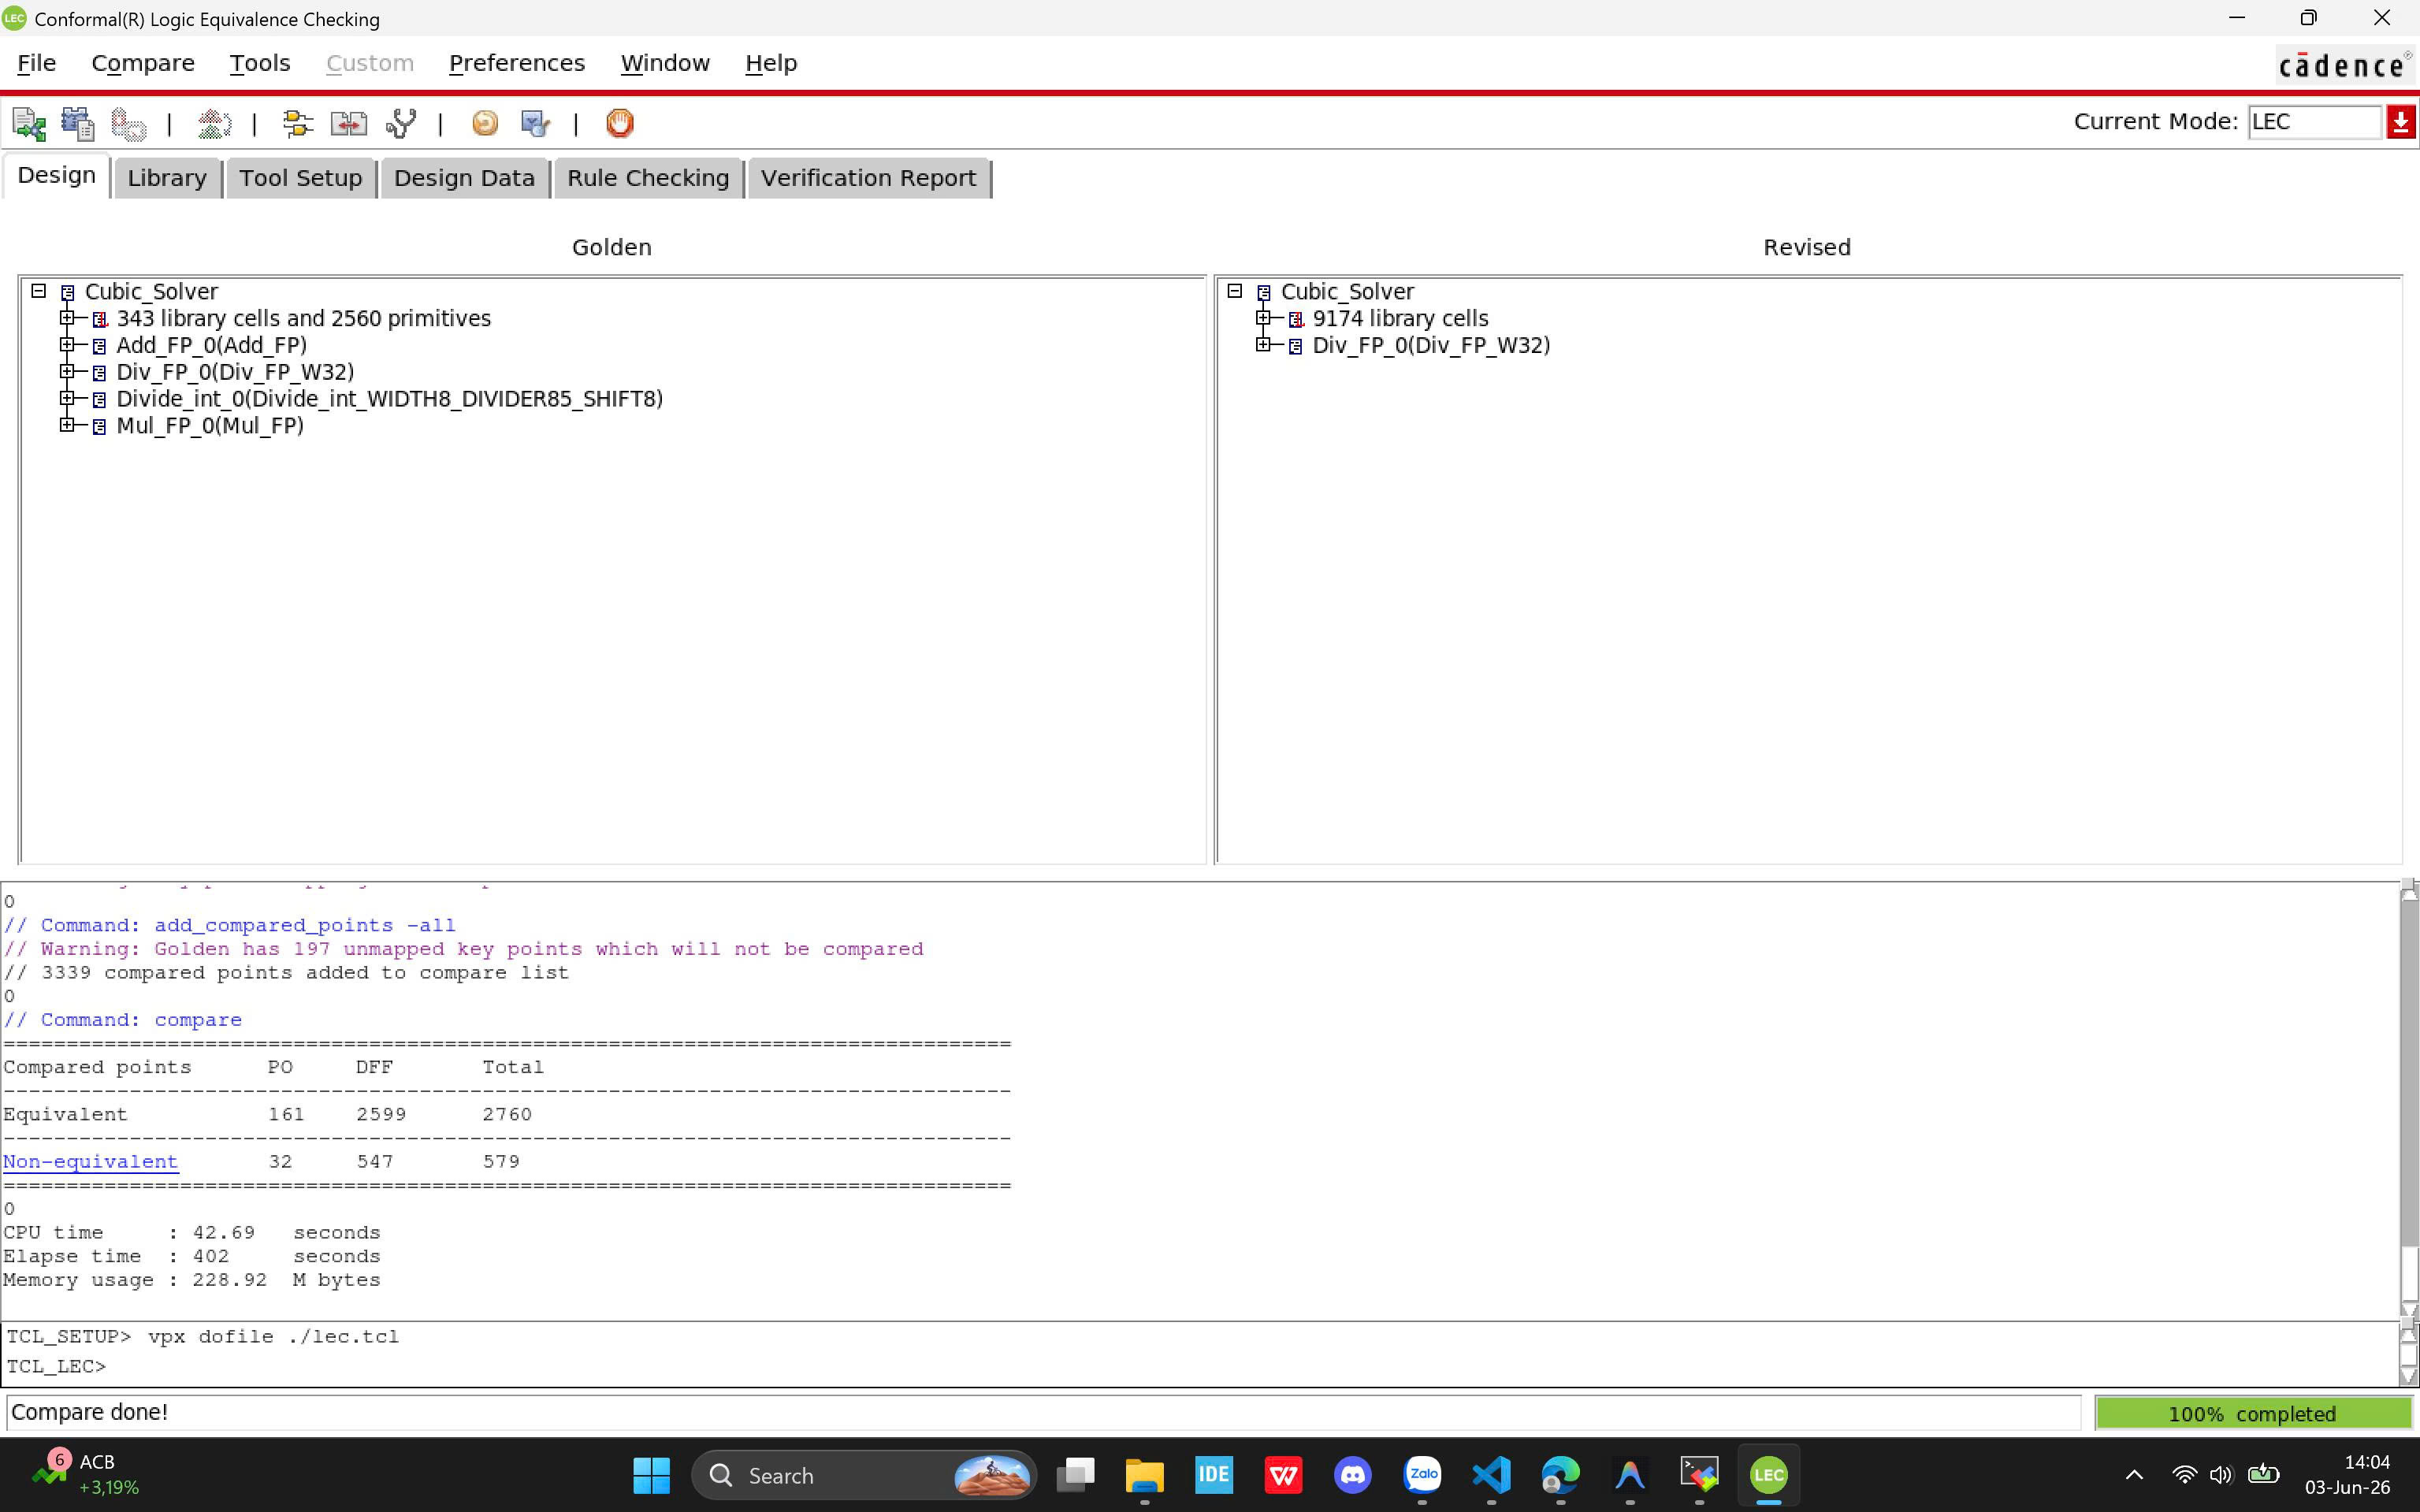
\includegraphics[width=0.8\textwidth]{graphics/synthesis_conformal/conformal_1.jpg}
    \caption{Conformal GUI}
    \label{fig:conformal_GUI}
\end{figure}    


\subsection{Key Point Mapping}
Before comparison, Conformal maps key points (Primary Inputs, Primary Outputs, and D-Flip-Flops) between the golden and revised designs. The mapping results are as follows:

\begin{table}[H]
\centering
\renewcommand{\arraystretch}{1.2}
\begin{tabular}{lrrrr}
\toprule
\textbf{Design} & \textbf{PI} & \textbf{PO} & \textbf{DFF} & \textbf{Total Mapped} \\
\midrule
Golden & 131 & 193 & 3146 & 3470 \\
Revised & 131 & 193 & 3146 & 3470 \\
\bottomrule
\end{tabular}
\caption{Mapped Key Points in Conformal LEC}
\label{tab:mapped_points}
\end{table}

Additionally, the golden design contains 549 unmapped points (352 unreachable and 197 not-mapped), which resulted in an incomplete key point mapping warning.

\subsection{Comparison Results}
After mapping, a total of 3339 key points were compared. The comparison phase yielded the following results:

\begin{table}[H]
\centering
\renewcommand{\arraystretch}{1.2}
\begin{tabular}{lrrr}
\toprule
\textbf{Status} & \textbf{PO} & \textbf{DFF} & \textbf{Total} \\
\midrule
Equivalent & 161 & 2599 & 2760 \\
Non-equivalent & 32 & 547 & 579 \\
\bottomrule
\end{tabular}
\caption{Comparison Results from Conformal LEC}
\label{tab:compare_results}
\end{table}
\subsection{Conformal mapping}
\begin{figure}[H]
    \centering
    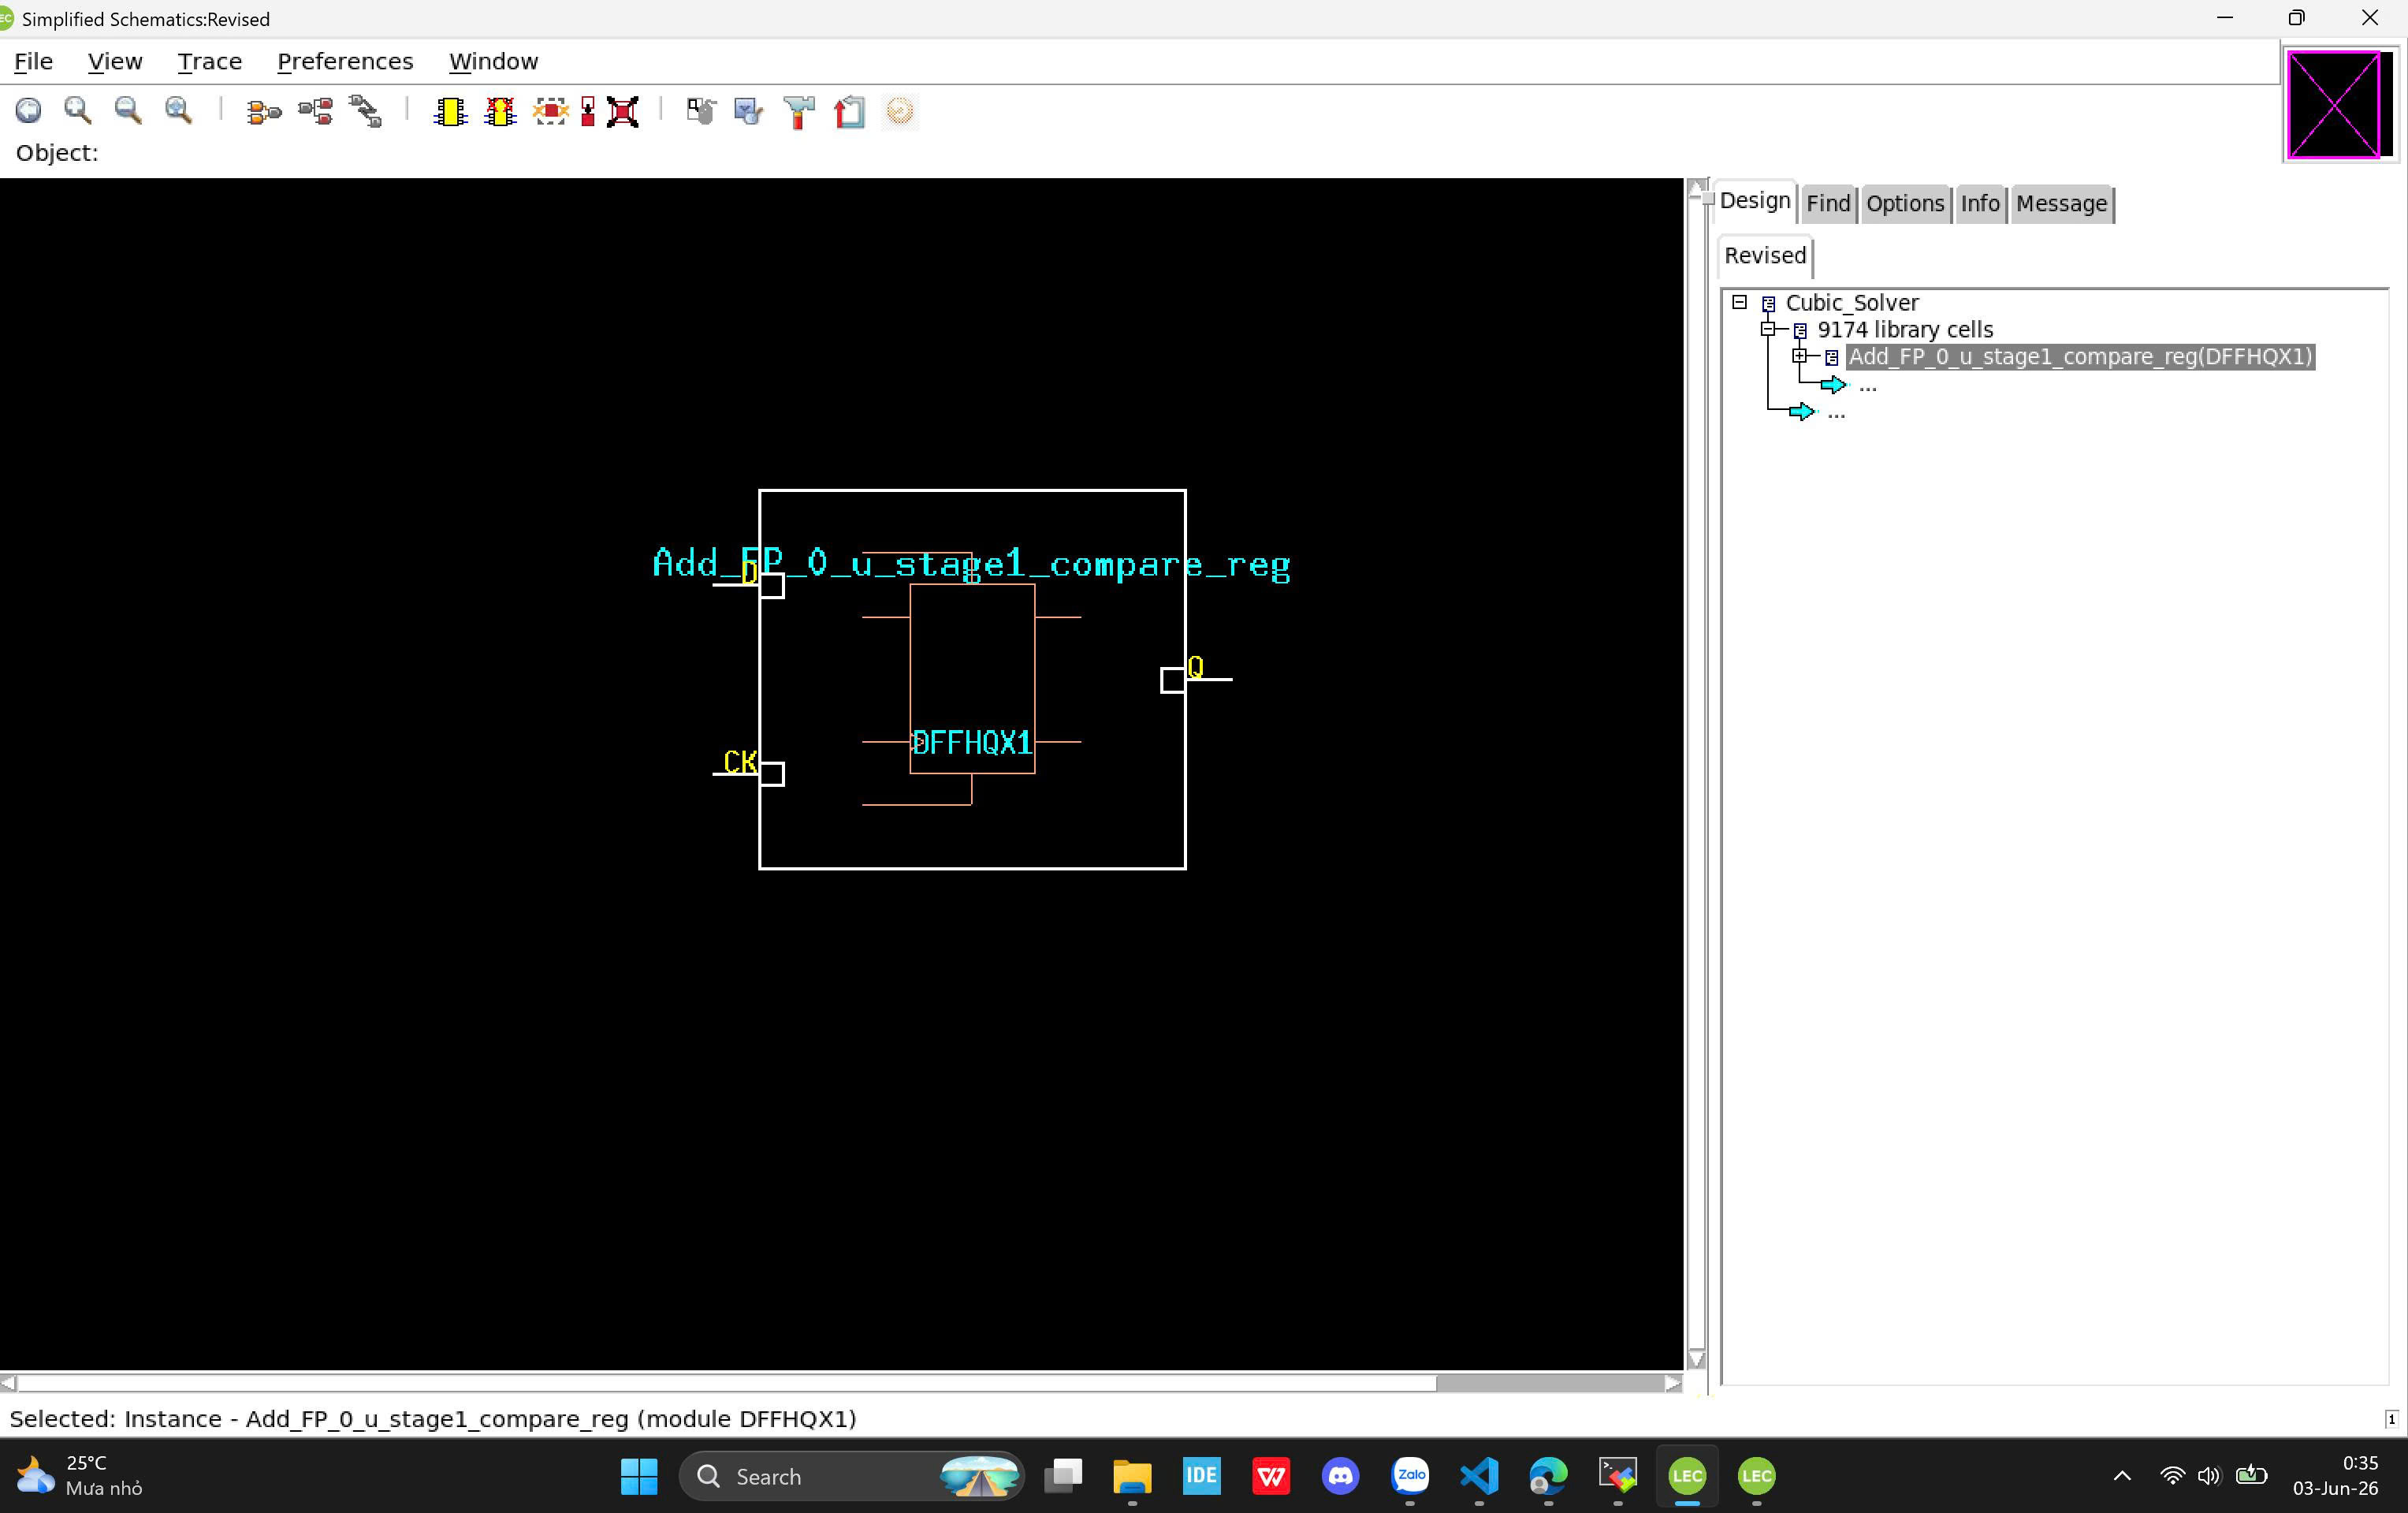
\includegraphics[width=0.8\textwidth]{graphics/synthesis_conformal/conformal_2.jpg}
    \caption{Conformal Schematic}
    \label{fig:conformal_mapping}
\end{figure}
\begin{figure}[H]
    \centering
    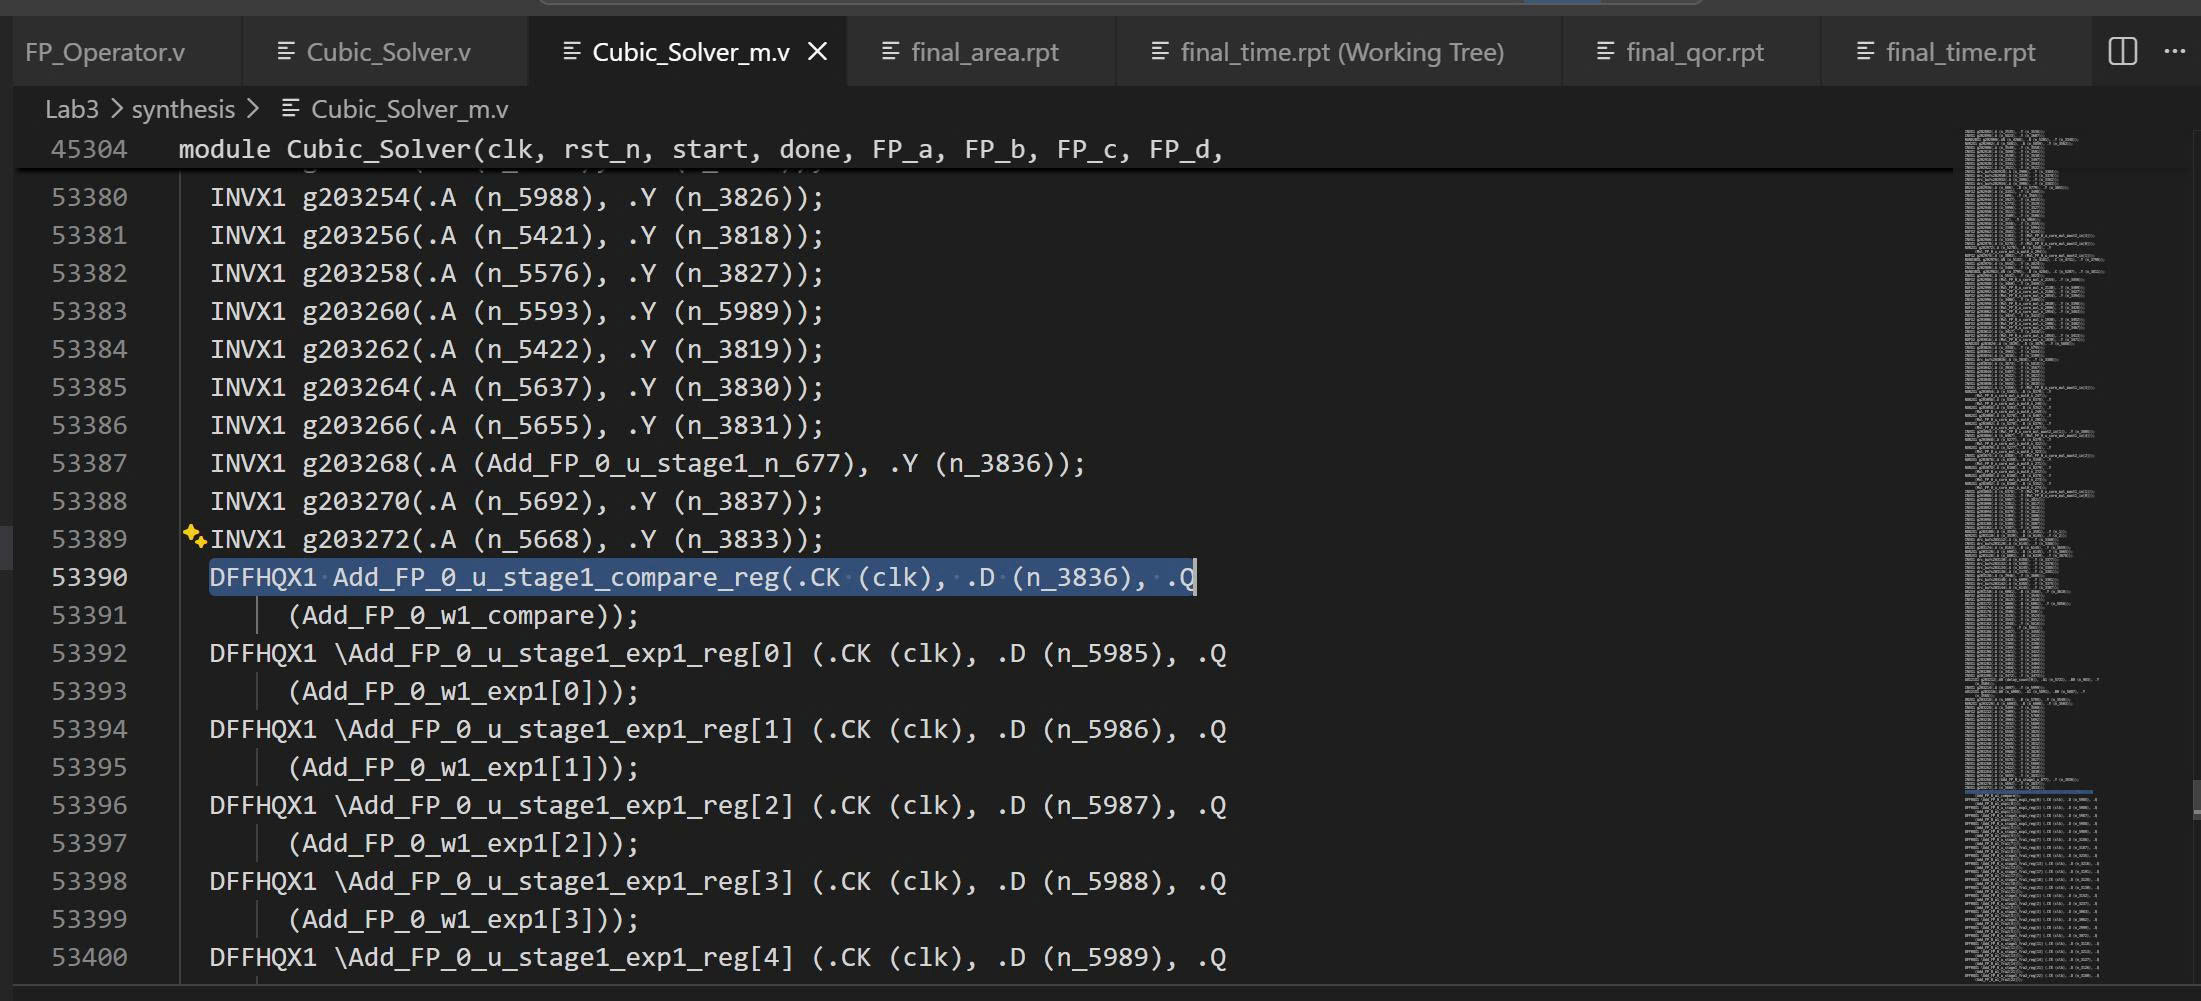
\includegraphics[width=0.8\textwidth]{graphics/synthesis_conformal/conformal_3.jpg}
    \caption{Netlist code}
    \label{fig:netlist_code}
\end{figure}
\subsection{Conclusion}
The formal verification process indicates that the golden RTL and the revised netlist are \textbf{NOT equivalent}. Out of the 3339 compared points, 579 points (32 Primary Outputs and 547 D-Flip-Flops) were found to be non-equivalent. Furthermore, 197 unmapped key points in the golden design were excluded from the comparison. 

This mismatch suggests that there may be issues in the synthesis constraints, unimplemented logic, or optimization mismatches that need to be resolved. Further debugging within Conformal is required to trace the non-equivalent points and ensure functional correctness of the synthesized netlist.
